% !TEX root = ../main.tex
\subsubsection{Conclusions}
\label{12.44::conclusions}

    \begin{figure}[b]
        \frame{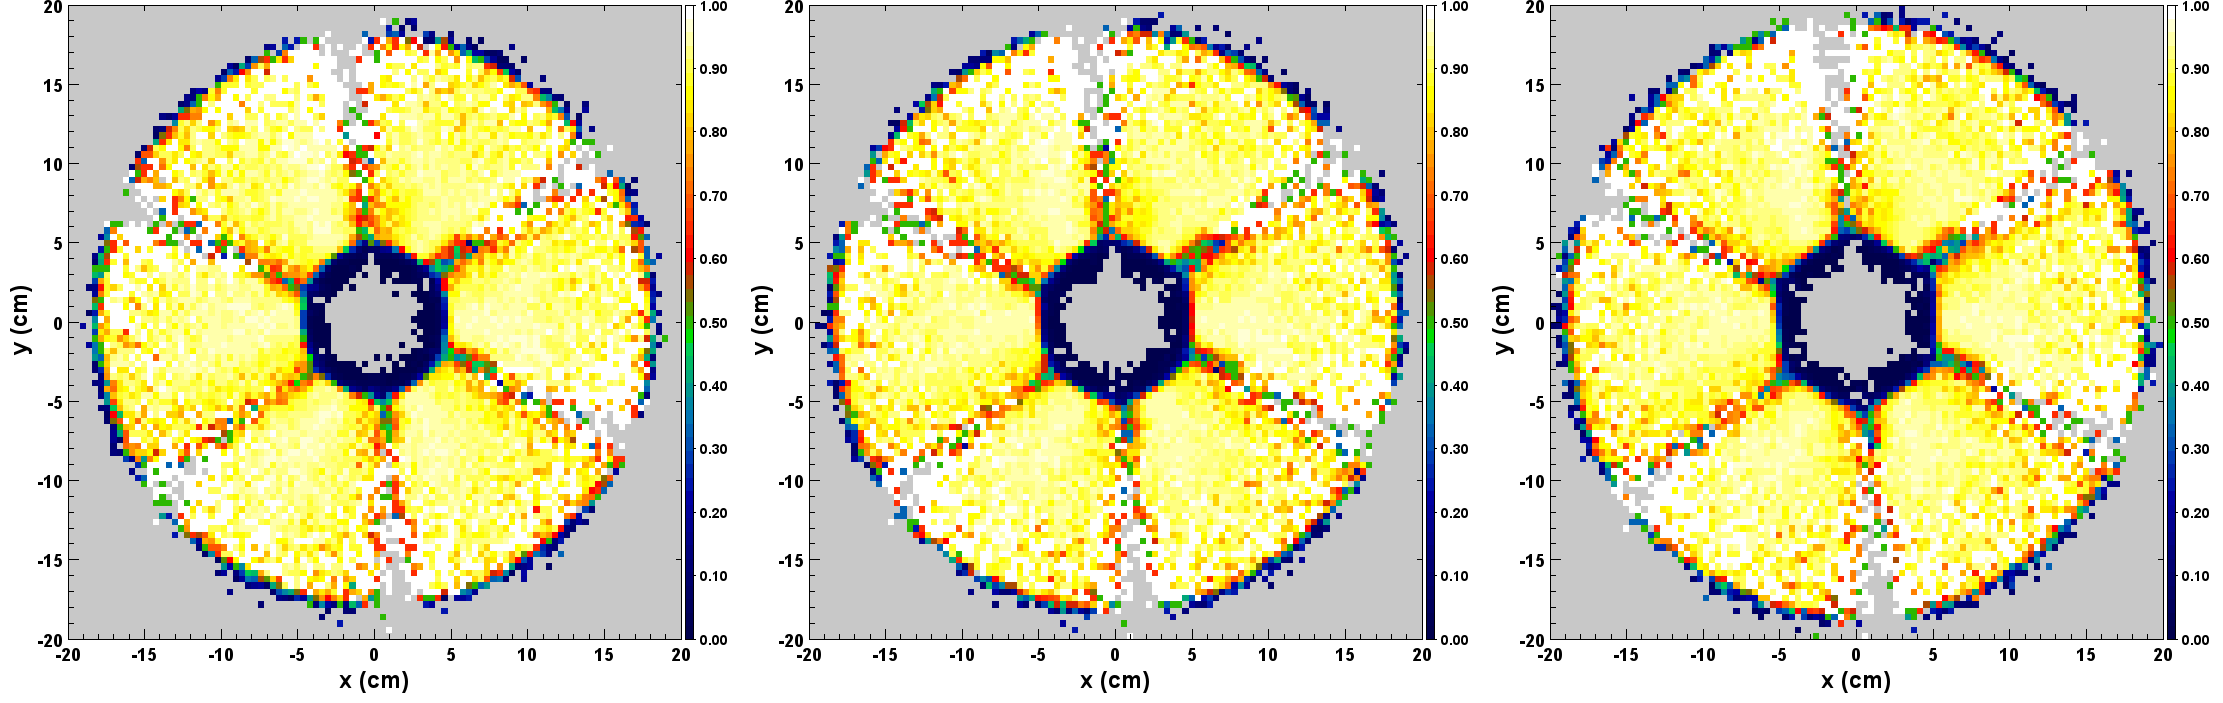
\includegraphics[width=\textwidth]{44fmt_efficiency.png}}
        \caption[FMT layers efficiency]
        {Efficiency of each FMT layer.}
        \floatfoot{Source: Own elaboration, using the \texttt{fmtVertex.groovy} script in \href{https://github.com/JeffersonLab/clas12alignment}{CLAS12 alignment software}.}
        \label{fig::12.44::fmt_azimuthal_efficiency}
    \end{figure}

    Although the improvement in resolution is not as significant as initially anticipated for the detector, it remains an encouraging result.
    The enhanced resolution enables more precise measurements of the target position.
    As a practical implication, it allows for double targets to be positioned closer to each other, thereby benefiting the derived physics from experiments like the RG-E run.

    The reason for the smaller-than-predicted improvement in resolution can be attributed to the initial projection, which assumed the presence of six FMT layers.
    The inclusion of six layers would provide additional positional data along the particle's track, thereby enhancing the accuracy of the vertex position measurement during the fitting process.

% --+ Why no improvements is seen on vertex momentum resolution +---------------
    Furthermore, due to the limited number of layers and their close proximity in the FMT detector, it exhibits a small lever arm.
    As a result, the detector's contribution to the vertex momentum resolution is not significant, as it does not provide sufficient additional data to accurately determine the track's momentum.

% --+ Show detector efficiency +------------------------------------------------
    In order to gain a better understanding of the FMT detector, we conducted a brief study on its efficiency.
    The efficiency is defined as the ratio of the number of FMT tracks to the number of DC tracks, representing how many of the DC tracks were also detected by the FMT.

    For the three-layer configuration, the efficiency is approximately $88.96\%$.
    Figure \ref{fig::12.44::fmt_azimuthal_efficiency} illustrates the layer-by-layer efficiency, showing no anomalous geometric effects.
    The observed gaps in efficiency are solely a result of the CLAS12 detector's geometry, which is divided into six sectors.
